\documentclass{extbook}[14pt]
\usepackage{multicol, enumerate, enumitem, hyperref, color, soul, setspace, parskip, fancyhdr, amssymb, amsthm, amsmath, bbm, latexsym, units, mathtools}
\everymath{\displaystyle}
\usepackage[headsep=0.5cm,headheight=0cm, left=1 in,right= 1 in,top= 1 in,bottom= 1 in]{geometry}
\usepackage{dashrule}  % Package to use the command below to create lines between items
\newcommand{\litem}[1]{\item #1

\rule{\textwidth}{0.4pt}}
\pagestyle{fancy}
\lhead{}
\chead{Answer Key for Progress Quiz 4 Version C}
\rhead{}
\lfoot{8448-1521}
\cfoot{}
\rfoot{Fall 2020}
\begin{document}
\textbf{This key should allow you to understand why you choose the option you did (beyond just getting a question right or wrong). \href{https://xronos.clas.ufl.edu/mac1105spring2020/courseDescriptionAndMisc/Exams/LearningFromResults}{More instructions on how to use this key can be found here}.}

\textbf{If you have a suggestion to make the keys better, \href{https://forms.gle/CZkbZmPbC9XALEE88}{please fill out the short survey here}.}

\textit{Note: This key is auto-generated and may contain issues and/or errors. The keys are reviewed after each exam to ensure grading is done accurately. If there are issues (like duplicate options), they are noted in the offline gradebook. The keys are a work-in-progress to give students as many resources to improve as possible.}

\rule{\textwidth}{0.4pt}

\begin{enumerate}\litem{
Determine the domain of the function below.
\[ f(x) = \frac{4}{24x^{2} -54 x + 30} \]
The solution is \( \text{All Real numbers except } x = 1.000 \text{ and } x = 1.250. \), which is option D.\begin{enumerate}[label=\Alph*.]
\item \( \text{All Real numbers.} \)

This corresponds to thinking the denominator has complex roots or that rational functions have a domain of all Real numbers.
\item \( \text{All Real numbers except } x = a, \text{ where } a \in [19.76, 20.41] \)

All Real numbers except $x = 20.000$, which corresponds to removing a distractor value from the denominator.
\item \( \text{All Real numbers except } x = a \text{ and } x = b, \text{ where } a \in [19.76, 20.41] \text{ and } b \in [34.9, 36.59] \)

All Real numbers except $x = 20.000$ and $x = 36.000$, which corresponds to not factoring the denominator correctly.
\item \( \text{All Real numbers except } x = a \text{ and } x = b, \text{ where } a \in [0.39, 1.05] \text{ and } b \in [1.12, 1.67] \)

All Real numbers except $x = 1.000$ and $x = 1.250$, which is the correct option.
\item \( \text{All Real numbers except } x = a, \text{ where } a \in [0.39, 1.05] \)

All Real numbers except $x = 1.000$, which corresponds to removing only 1 value from the denominator.
\end{enumerate}

\textbf{General Comment:} Recall that dividing by zero is not a real number. Therefore the domain is all real numbers \textbf{except} those that make the denominator 0.
}
\litem{
Solve the rational equation below. Then, choose the interval(s) that the solution(s) belongs to.
\[ \frac{-4x}{-3x -7} + \frac{-2x^{2}}{15x^{2} +56 x + 49} = \frac{-7}{-5x -7} \]
The solution is \( \text{There are two solutions: } x = 1.467 \text{ and } x = -1.856 \), which is option A.\begin{enumerate}[label=\Alph*.]
\item \( x_1 \in [1.34, 1.76] \text{ and } x_2 \in [-2.21,-1.38] \)

* $x = 1.467 \text{ and } x = -1.856$, which is the correct option.
\item \( \text{All solutions lead to invalid or complex values in the equation.} \)


\item \( x_1 \in [1.34, 1.76] \text{ and } x_2 \in [-2.48,-2.09] \)


\item \( x \in [-2.4,-1.65] \)


\item \( x \in [-1.44,-1.29] \)


\end{enumerate}

\textbf{General Comment:} Distractors are different based on the number of solutions. Remember that after solving, we need to make sure our solution does not make the original equation divide by zero!
}
\litem{
Solve the rational equation below. Then, choose the interval(s) that the solution(s) belongs to.
\[ \frac{-6}{-3x + 2} + 7 = \frac{4}{9x -6} \]
The solution is \( x = 0.444 \), which is option E.\begin{enumerate}[label=\Alph*.]
\item \( x_1 \in [-1.27, -0.51] \text{ and } x_2 \in [-0.56,2.44] \)

$x = -0.889 \text{ and } x = 0.444$, which corresponds to getting the correct solution and believing there should be a second solution to the equation.
\item \( \text{All solutions lead to invalid or complex values in the equation.} \)

This corresponds to thinking $x = 0.444$ leads to dividing by zero in the original equation, which it does not.
\item \( x \in [-1.27,-0.51] \)

$x = -0.889$, which corresponds to not distributing the factor $-3x + 2$ correctly when trying to eliminate the fraction.
\item \( x_1 \in [-0.41, 0.27] \text{ and } x_2 \in [-0.56,2.44] \)

$x = 0.190 \text{ and } x = 0.444$, which corresponds to getting the correct solution and believing there should be a second solution to the equation.
\item \( x \in [-0.56,1.44] \)

* $x = 0.444$, which is the correct option.
\end{enumerate}

\textbf{General Comment:} Distractors are different based on the number of solutions. Remember that after solving, we need to make sure our solution does not make the original equation divide by zero!
}
\litem{
Solve the rational equation below. Then, choose the interval(s) that the solution(s) belongs to.
\[ \frac{-42}{63x + 63} + 1 = \frac{-42}{63x + 63} \]
The solution is \( \text{all solutions are invalid or lead to complex values in the equation.} \), which is option C.\begin{enumerate}[label=\Alph*.]
\item \( x \in [-1.0,1.0] \)

$x = -1.000$, which corresponds to not checking if this value leads to dividing by 0 in the original equation and thus is not a valid solution.
\item \( x_1 \in [-1, 0] \text{ and } x_2 \in [-2.2,-0.9] \)

$x = -1.000 \text{ and } x = -1.000$, which corresponds to getting the correct solution and believing there should be a second solution to the equation.
\item \( \text{All solutions lead to invalid or complex values in the equation.} \)

*$x = -1.000$ leads to dividing by 0 in the original equation and thus is not a valid solution, which is the correct option.
\item \( x \in [1,2] \)

$x = 1.000$, which corresponds to not distributing the factor $63x + 63$ correctly when trying to eliminate the fraction.
\item \( x_1 \in [-1, 0] \text{ and } x_2 \in [0.1,1.6] \)

$x = -1.000 \text{ and } x = 1.000$, which corresponds to getting the correct solution and believing there should be a second solution to the equation.
\end{enumerate}

\textbf{General Comment:} Distractors are different based on the number of solutions. Remember that after solving, we need to make sure our solution does not make the original equation divide by zero!
}
\litem{
Determine the domain of the function below.
\[ f(x) = \frac{3}{30x^{2} +54 x + 24} \]
The solution is \( \text{All Real numbers except } x = -1.000 \text{ and } x = -0.800. \), which is option B.\begin{enumerate}[label=\Alph*.]
\item \( \text{All Real numbers.} \)

This corresponds to thinking the denominator has complex roots or that rational functions have a domain of all Real numbers.
\item \( \text{All Real numbers except } x = a \text{ and } x = b, \text{ where } a \in [-1.12, -0.94] \text{ and } b \in [-0.83, -0.59] \)

All Real numbers except $x = -1.000$ and $x = -0.800$, which is the correct option.
\item \( \text{All Real numbers except } x = a \text{ and } x = b, \text{ where } a \in [-36.15, -35.93] \text{ and } b \in [-20.04, -19.83] \)

All Real numbers except $x = -36.000$ and $x = -20.000$, which corresponds to not factoring the denominator correctly.
\item \( \text{All Real numbers except } x = a, \text{ where } a \in [-1.12, -0.94] \)

All Real numbers except $x = -1.000$, which corresponds to removing only 1 value from the denominator.
\item \( \text{All Real numbers except } x = a, \text{ where } a \in [-36.15, -35.93] \)

All Real numbers except $x = -36.000$, which corresponds to removing a distractor value from the denominator.
\end{enumerate}

\textbf{General Comment:} Recall that dividing by zero is not a real number. Therefore the domain is all real numbers \textbf{except} those that make the denominator 0.
}
\litem{
Choose the graph of the equation below.
\[ f(x) = \frac{1}{(x - 1)^2} - 3 \]
The solution is the graph below, which is option B.
\begin{center}
    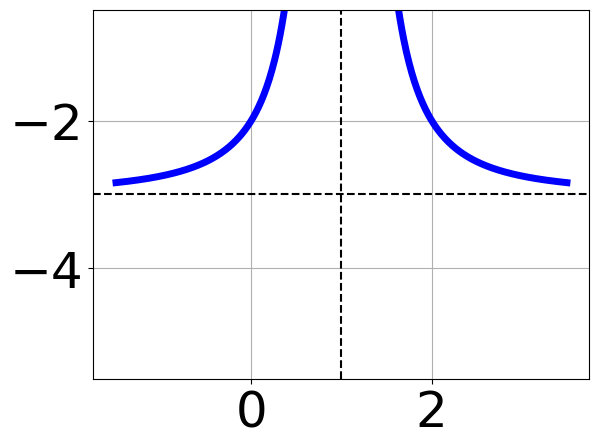
\includegraphics[width=0.3\textwidth]{../Figures/rationalEquationToGraphBC.png}
\end{center}\begin{enumerate}[label=\Alph*.]
\begin{multicols}{2}
\item 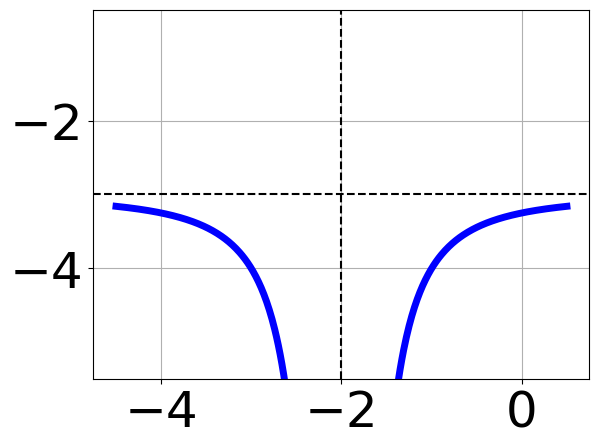
\includegraphics[width = 0.3\textwidth]{../Figures/rationalEquationToGraphAC.png}
\item 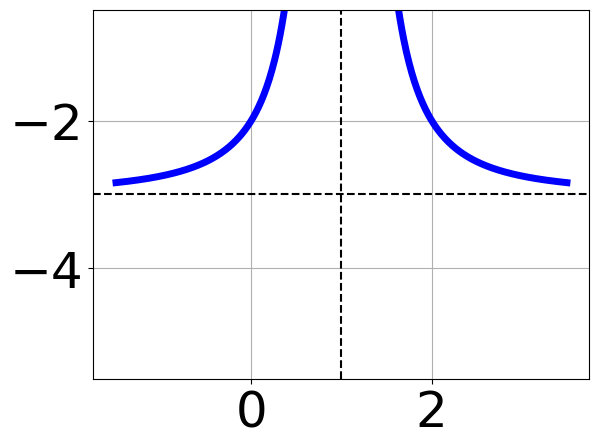
\includegraphics[width = 0.3\textwidth]{../Figures/rationalEquationToGraphBC.png}
\item 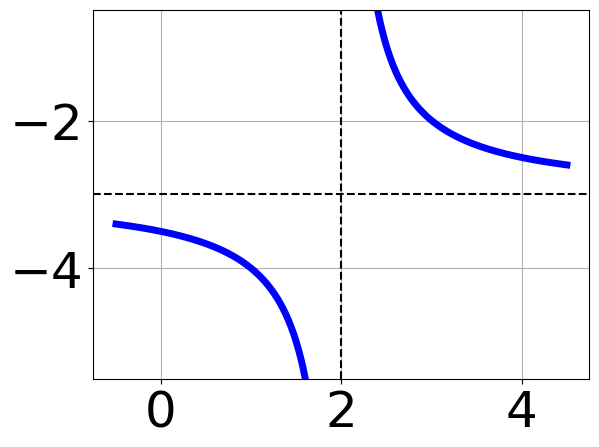
\includegraphics[width = 0.3\textwidth]{../Figures/rationalEquationToGraphCC.png}
\item 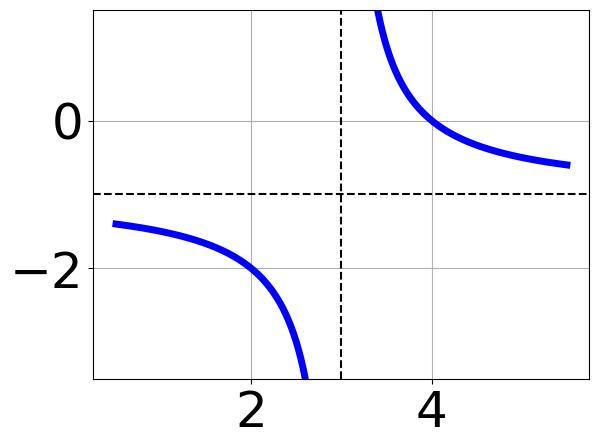
\includegraphics[width = 0.3\textwidth]{../Figures/rationalEquationToGraphDC.png}
\end{multicols}\item None of the above.\end{enumerate}
\textbf{General Comment:} Remember that the general form of a basic rational equation is $ f(x) = \frac{a}{(x-h)^n} + k$, where $a$ is the leading coefficient (and in this case, we assume is either $1$ or $-1$), $n$ is the degree (in this case, either $1$ or $2$), and $(h, k)$ is the intersection of the asymptotes.
}
\litem{
Solve the rational equation below. Then, choose the interval(s) that the solution(s) belongs to.
\[ \frac{-4x}{-7x + 3} + \frac{-3x^{2}}{28x^{2} -61 x + 21} = \frac{-3}{-4x + 7} \]
The solution is \( \text{There are two solutions: } x = 0.194 \text{ and } x = 3.576 \), which is option C.\begin{enumerate}[label=\Alph*.]
\item \( x_1 \in [-2.31, 0.25] \text{ and } x_2 \in [-1.57,2.43] \)


\item \( x \in [3.37,4.36] \)


\item \( x_1 \in [-2.31, 0.25] \text{ and } x_2 \in [0.58,6.58] \)

* $x = 0.194 \text{ and } x = 3.576$, which is the correct option.
\item \( \text{All solutions lead to invalid or complex values in the equation.} \)


\item \( x \in [1.34,2.03] \)


\end{enumerate}

\textbf{General Comment:} Distractors are different based on the number of solutions. Remember that after solving, we need to make sure our solution does not make the original equation divide by zero!
}
\litem{
Choose the equation of the function graphed below.

\begin{center}
    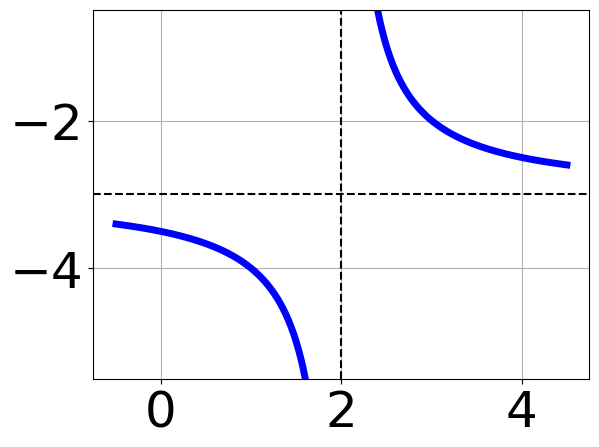
\includegraphics[width=0.5\textwidth]{../Figures/rationalGraphToEquationC.png}
\end{center}



The solution is \( f(x) = \frac{1}{x - 2} - 3 \), which is option C.\begin{enumerate}[label=\Alph*.]
\item \( f(x) = \frac{1}{(x - 2)^2} - 3 \)

Corresponds to thinking the graph was a shifted version of $\frac{1}{x^2}$.
\item \( f(x) = \frac{-1}{x + 2} - 3 \)

Corresponds to using the general form $f(x) = \frac{a}{x+h}+k$ and the opposite leading coefficient.
\item \( f(x) = \frac{1}{x - 2} - 3 \)

This is the correct option.
\item \( f(x) = \frac{-1}{(x + 2)^2} - 3 \)

Corresponds to thinking the graph was a shifted version of $\frac{1}{x^2}$, using the general form $f(x) = \frac{a}{x+h}+k$, and the opposite leading coefficient.
\item \( \text{None of the above} \)

This corresponds to believing the vertex of the graph was not correct.
\end{enumerate}

\textbf{General Comment:} Remember that the general form of a basic rational equation is $ f(x) = \frac{a}{(x-h)^n} + k$, where $a$ is the leading coefficient (and in this case, we assume is either $1$ or $-1$), $n$ is the degree (in this case, either $1$ or $2$), and $(h, k)$ is the intersection of the asymptotes.
}
\litem{
Choose the graph of the equation below.
\[ f(x) = \frac{-1}{x + 2} + 3 \]
The solution is the graph below, which is option E.
\begin{center}
    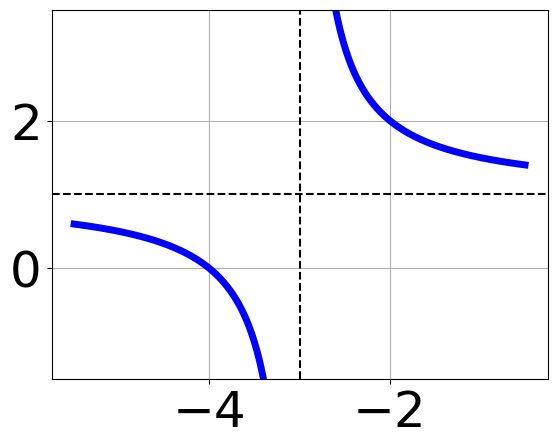
\includegraphics[width=0.3\textwidth]{../Figures/rationalEquationToGraphCopyEC.png}
\end{center}\begin{enumerate}[label=\Alph*.]
\begin{multicols}{2}
\item 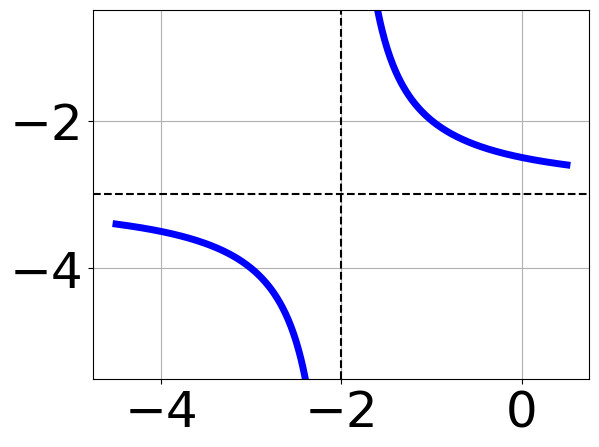
\includegraphics[width = 0.3\textwidth]{../Figures/rationalEquationToGraphCopyAC.png}
\item 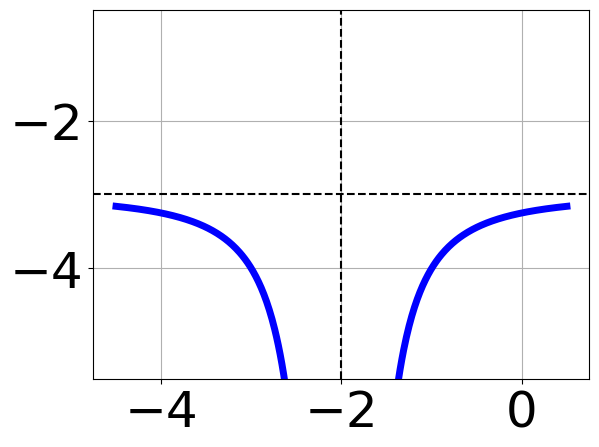
\includegraphics[width = 0.3\textwidth]{../Figures/rationalEquationToGraphCopyBC.png}
\item 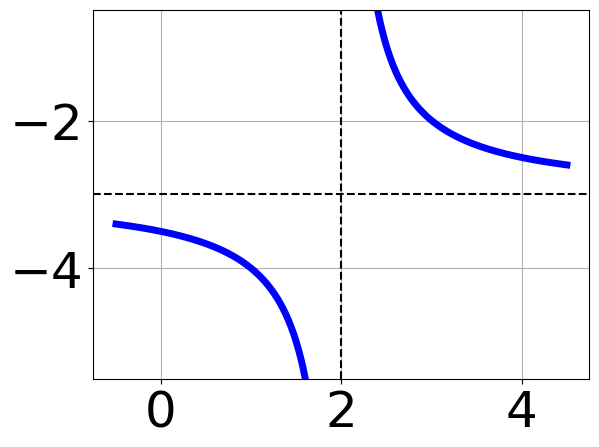
\includegraphics[width = 0.3\textwidth]{../Figures/rationalEquationToGraphCopyCC.png}
\item 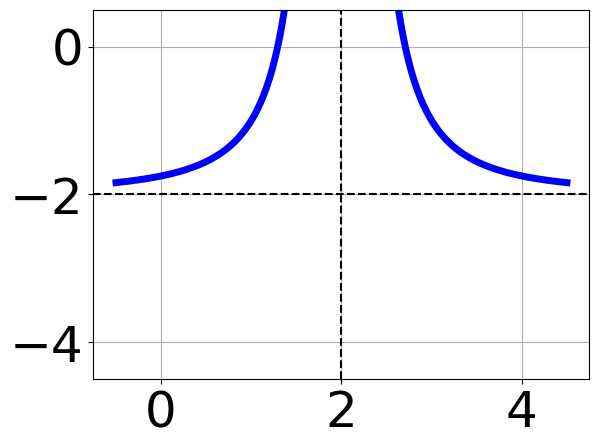
\includegraphics[width = 0.3\textwidth]{../Figures/rationalEquationToGraphCopyDC.png}
\end{multicols}\item None of the above.\end{enumerate}
\textbf{General Comment:} Remember that the general form of a basic rational equation is $ f(x) = \frac{a}{(x-h)^n} + k$, where $a$ is the leading coefficient (and in this case, we assume is either $1$ or $-1$), $n$ is the degree (in this case, either $1$ or $2$), and $(h, k)$ is the intersection of the asymptotes.
}
\litem{
Choose the equation of the function graphed below.

\begin{center}
    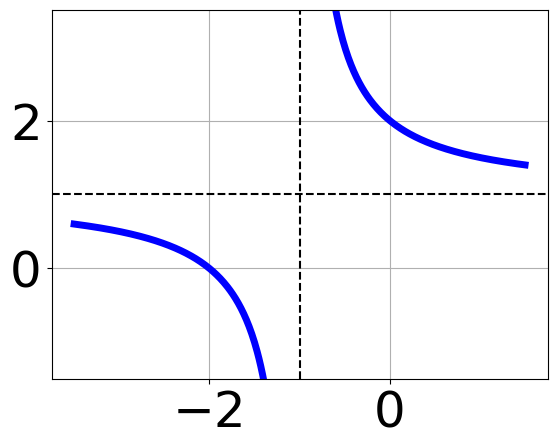
\includegraphics[width=0.5\textwidth]{../Figures/rationalGraphToEquationCopyC.png}
\end{center}



The solution is \( \text{None of the above as it should be } f(x) = \frac{1}{x + 1} + 1 \), which is option E.\begin{enumerate}[label=\Alph*.]
\item \( f(x) = \frac{1}{x - 1} + 1 \)

The $x$-value of the equation does not match the graph.
\item \( f(x) = \frac{-1}{(x + 1)^2} + 1 \)

Corresponds to thinking the graph was a shifted version of $\frac{1}{x^2}$, using the general form $f(x) = \frac{a}{x-h}+k$, and the opposite leading coefficient.
\item \( f(x) = \frac{-1}{x + 1} + 1 \)

Corresponds to using the general form $f(x) = \frac{a}{x-h}+k$ and the opposite leading coefficient.
\item \( f(x) = \frac{1}{(x - 1)^2} + 1 \)

Corresponds to thinking the graph was a shifted version of $\frac{1}{x^2}$.
\item \( \text{None of the above} \)

None of the equation options were the correct equation.
\end{enumerate}

\textbf{General Comment:} Remember that the general form of a basic rational equation is $ f(x) = \frac{a}{(x-h)^n} + k$, where $a$ is the leading coefficient (and in this case, we assume is either $1$ or $-1$), $n$ is the degree (in this case, either $1$ or $2$), and $(h, k)$ is the intersection of the asymptotes.
}
\end{enumerate}

\end{document}